\begin{greek}
\chapter{Συλλογή σκουπιδιών με σήμανση και συμπύκνωση}\label{ch:mrkcmp}
Η τάση τους να κατακερματίζουν τη μνήμη είναι το βασικό πρόβλημα των μη-μετακινούντων 
συλλεκτών σκουπιδιών. Παρότι μπορεί να υπάρχει ελεύθερη μνήμη στο σωρό, αυτή είναι 
πολύ πιθανόν να είναι κατακερματισμένη  σε πολλά μικρά τμήματα και όχι συνεχόμενη. 
Συνεπώς είναι πιθανόν ο εκχωρητής να μην ικανοποιήσει ένα αίτημα παρότι υπάρχει
ελεύθερη μνήμη στο σωρό καθώς αυτή είναι κατακερματισμένη.

Η \textbf{συλλογή σκουπιδιών με σήμανση και συμπύκνωση} επινοήθηκε προς λύσιν του προβλήματος του κατακερματισμού. 
Το σημαντικό πλεονέκτημα της μεθόδου είναι πώς απλοποιεί το έργο του εκχωρητή. Ο σωρός 
αποτελείται από δύο συνεχόμενα τμήματα: το πρώτο φιλοξενεί αντικείμενα ενώ το δεύτερο 
είναι ελεύθερο και χρησιμοποιείται από τον εκχωρητή για την ικανοποίηση αιτημάτων μνήμης. 
Τα δύο αυτά τμήματα διαχωρίζονται από ένα δείκτη, ο οποίος σηματοδοτεί ταυτόχρονα το 
τέλος του χρησιμοποιούμενου τμήματος και την αρχή του ελεύθερου τμήματος. Συνεπώς, αν 
υπάρχει ελεύθερη μνήμη (πρακτικά αν ο εν λόγω δείκτης δεν έχει ξεπεράσει το τέλος του 
σωρού), ο εκχωρητής επιστρέφει την τιμή του δείκτη και κατόπιν τον ενημερώνει αυξάνοντας
τον κατά το μέγεθος του αιτήματος. Η συλλογή με σήμανση και συμπύκνωση συγκεντρώνει τα 
προσβάσιμα αντικείμενα στο άκρο του σωρού, ο οποίος είναι ενιαίος. Αντίθετα, η συλλογή 
με αντιγραφή  την οποία εξετάζουμε στο επόμενο κεφάλαιο μετακινεί τα προσβάσιμα 
αντικείμενα από έναν ημιχώρο σε έναν άλλο ημιχώρο του σωρού.

Οι συλλέκτες με σήμανση και συμπύκνωση λειτουργούν σε φάσεις. Η πρώτη φάση είναι πάντα 
αυτή της σήμανσης, την οποία και εξετάσαμε στο προηγούμενο κεφάλαιο. Τη φάση της σήμανσης 
διαδέχονται οι φάσεις της συμπύκνωσης, οι οποίες μετακινούν αντικείμενα και ενημερώνουν 
τις μεταβλητές δείκτες που δείχνουν σε προσβάσιμα αντικείμενα με τις νέες διευθύνσεις 
αυτών. Το πλήθος των φάσεων, η σειρά με την οποία αυτές εκτελούνται καθώς και ο τρόπος με 
τον οποίο μετακινούνται τα αντικείμενα διαφέρει από αλγόριθμο σε αλγόριθμο. Ο τρόπος 
μάλιστα με τον οποίο συμπυκνώνονται τα αντικείμενα επηρεάζει την τοπικότητα του 
τροποποιητή.

Κάθε μετακινών συλλέκτης μπορεί να οργανώσει τα αντικείμενα στο σωρό με έναν από τους 
ακόλουθους 3 τρόπους, οπότε και χαρακτηρίζεται ως:
\begin{enumerate}
\item \textbf{τυχαίoς (arbitrary)}: Τα αντικείμενα μετακινούνται ανεξαρτήτως της αρχικής 
      τους σειράς ή του αν δείχνουν το ένα στο άλλο. 
\item \textbf{γραμμικοποιών (linearising)}: Τα αντικείμενα τοποθετούνται με τέτοιο 
      τρόπο ώστε να είναι κοντά με σχετικά προς αυτά αντικείμενα στο μέγιστο βαθμό. Δύο 
      αντικείμενα είναι σχετικά αν το ένα δείχνει στο άλλο ή αν είναι αδέρφια σε μια 
      δομή δεδομένων κ.ο.κ.
\item \textbf{ολισθαίνων (sliding)}: Τα αντικείμενα ``ολισθαίνουν'' στο ένα άκρο του 
      σωρού, με αποτέλεσμα να διατηρείται η αρχική τους διάταξη στο σωρό. 
\end{enumerate}

Οι περισσότεροι συλλέκτες με σήμανση και συμπύκνωση που απαντώνται στη βιβλιογραφία είναι 
τυχαίοι ή ολισθαίνοντες. Οι συλλέκτες αυτών των κατηγοριών έχουν απλή υλοποίηση και 
εξαιρετικές επιδόσεις σε ταχύτητα. Το μειονέκτημά τους είναι πώς οδηγούν σε μικρή έως 
καθόλου τοπικότητα για τον τροποποιητή, καθώς αντικείμενα αντιστοιχίζονται σε διαφορετικά 
μπλοκ της μνήμης cache ή ακόμα και σε διαφορετικές σελίδες της εικονικής μνήμης. Ο 
Abuaiadh κ.ά  σε πρόσφατη μελέτη τους, \cite{DBLP:conf/oopsla/AbuaiadhOPS04} επαληθεύουν 
πώς η τυχαία συμπύκνωση του σωρού μπορεί να οδηγήσει σε δραστική μείωση της διεκπεραιωτικής 
ικανότητας του τροποποιητή. Όλοι οι σύγχρονοι συλλέκτες με σήμανση και συμπύκνωση είναι 
ολισθαίνοντες και έτσι δεν παρεμβαίνουν στην τοπικότητα του τροποποιητή.

Οι τυχαίοι συλλέκτες διαχειρίζονται αντικείμενα ενός συγκεκριμένου μεγέθους ή συμπυκνώνουν 
ξεχωριστά αντικείμενα διαφορετικών μεγεθών. Η συμπύκνωση μπορεί να απαιτεί δύο ή τρία 
περάσματα στο σωρό. Ακόμη ενδέχεται να χρειάζεται η προσθήκη μιας επιπλέον λέξης στην 
επικεφαλίδα ενός αντικειμένου όπου θα αποθηκεύονται πληροφορίες σχετικά με τη νέα διεύθυνση 
του αυτού. Το κόστος σε χώρο από την προσθήκη αυτή μπορεί να είναι σημαντικό σε έναν γενικού 
σκοπού διαχειριστή μνήμης. Τέλος, οι συλλέκτες με συμπύκνωση μπορεί να επιβάλλουν 
επιπρόσθετους περιορισμούς όσον αφορά τις μεταβλητές δείκτες. Για παράδειγμα, σε προς ποια 
κατεύθυνση επιτρέπεται αυτοί να δείχνουν; Επιτρέπονται οι εσωτερικοί δείκτες;

Στη συνέχεια εξετάζουμε διάφορα είδη συμπύκνωσης. Σε κάθε περίπτωση, ο συλλέκτης καλείται 
ως εξής:

\begin{algorithm}
  \caption{Συλλογή με σήμανση και συμπύκνωση}
  \label{alg:mrkcmp}
  \begin{algorithmic}[1]
    \State \Call{markFromRoots}{\null}
    \State \Call{compact}{\null}
  \end{algorithmic}
\end{algorithm}

\section{Συμπύκνωση με δύο δείκτες}
Ο αλγόριθμος Two-Finger \cite{saunders1964lisp} εκτελεί τη συμπύκνωση σε δύο φάσεις και 
συμπυκνώνει τα προσβάσιμα αντικείμενα σε τυχαία σειρά. Είναι βέλτιστος δε στην ειδική 
περίπτωση όπου ο τροποποιητής χρησιμοποιεί τα αντικείμενα του ίδιου σταθερού μεγέθους. 
Η ιδέα του είναι απλή: δοθέντος του όγκου των προσβάσιμων αντικειμένων στην προς συμπύκνωση 
περιοχή, γνωρίζουμε ποιο θα είναι το όριο της περιοχής αυτής μετά την συμπύκνωση. Ζωντανά 
αντικείμενα πάνω από αυτό το κατώφλι αντιγράφονται στα κατάλληλα κενά κάτω  από το κατώφλι.

Ο αλγόριθμος διατηρεί δύο δείκτες, τους $free$ και $scan$, οι οποίοι αρχικά δείχνουν στην 
αρχή και το τέλος της προς συμπύκνωση περιοχής. Στη διάρκεια της πρώτης φάσης, ο δείκτης 
$free$ αυξάνεται μέχρις ότου συναντήσει ένα αντικείμενο που είναι ελεύθερο (μη-σημασμένο), 
ενώ ο δείκτης $scan$ μειώνεται μέχρις ότου συναντήσει ένα ζωντανό αντικείμενο (σημασμένο). 
Αν οι δύο δείκτες συναντηθούν, η πρώτη αυτή φάση ολοκληρώνεται. 

\begin{figure}[H]
  \centering
  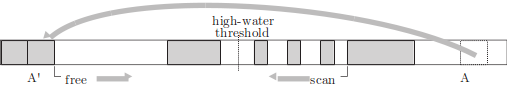
\includegraphics{figures/mrkcmp_1}
  \caption[Ο αλγόριθμος Two-Finger του Edward]
    {Ο αλγόριθμος Two-Finger του Edward. Ζωντανά αντικείμενα
     από την κορυφή του σωρού μετακινούνται σε ελεύθερα κενά
     στη βάση του σωρού. Εδώ το αντικείμενο στη θέση Α έχει
     μετακινηθεί στη θέση Α'. Ο αλγόριθμος τερματίζει όταν
     οι δείκτες $scan$ και $free$ συναντηθούν.}
  \label{fig:mrkcmp_1}
\end{figure}

\begin{algorithm}[H]
  \caption{Ο αλγόριθμος συμπύκνωσης Two-Finger}
  \label{alg:mrkcmp1}
  \begin{algorithmic}[1]
    \Procedure{compact}{\null}
      \State \Call{relocate}{$HeapStart$, $HeapEnd$}
      \State \Call{updateReferences}{$HeapStart$, $free$}
    \EndProcedure
    \Statex
    \Procedure{relocate}{$start$, $end$}
      \State $free \gets start$
      \State $scan \gets end$
      \While{$free < scan$}
        \While{\Call{isMarked}{$free$}}
          \State \Call{unsetMarked}{$free$}
          \State $free \gets free$ $+$ \Call{size}{$free$} \Comment{find next hole}
        \EndWhile
        \While{\textbf{not} \Call{isMarked}{$scan$} \textbf{and} $scan > free$}
          \State $scan \gets scan$ $-$ \Call{size}{$scan$} \Comment{find previous live object}
        \EndWhile
        \If{$scan > free$}
          \State \Call{unsetMarked}{$scan$}
          \State \Call{move}{$scan$, $free$}
          \State $scan \gets free$ \Comment{leave forwarding address (destructively)}
          \State $free \gets free$ $+$ \Call{size}{$free$}
          \State $scan \gets scan$ $-$ \Call{size}{$scan$}
        \EndIf
      \EndWhile
    \EndProcedure
    \Statex
    \Procedure{updateReferences}{$start$, $end$}
      \ForAll{$fld \; \textbf{in} \; Roots$} \Comment{update roots that pointed to moved objects}
        \State $ref \gets *fld$
        \If{$ref > end$}
          \State $*fld \gets ref$ %\Comment{use the forwarding address left in the first pass}
        \EndIf
      \EndFor
      \State $scan \gets start$
      \While{$scan < end$} \Comment{update fields in live region}
        \ForAll{$fld \; \textbf{in} \; Pointers(scan)$}
          \State $ref \gets *fld$
          \If{$ref > end$}
            \State $*fld \gets ref$ \Comment{use the forwarding address left in the first pass}
          \EndIf
        \EndFor
        \State $scan \gets scan$ $+$ \Call{size}{$scan$} \Comment{next object}
      \EndWhile
    \EndProcedure
  \end{algorithmic}
\end{algorithm}

Αλλιώς, το αντικείμενο στη 
θέση $scan$ αντιγράφεται στη θέση $free$, στο παλιό αντίγραφο στη θέση $scan$ αποθηκεύεται 
η νέα διεύθυνση (την τιμή του δείκτη $free$ εκείνη τη χρονική στιγμή) του αντικειμένου και 
η διαδικασία επαναλαμβάνεται. Είναι εμφανές πώς η ποιότητα της συμπύκνωσης εξαρτάται 
πρωτίστως από το εάν το μέγεθος του αντικειμένου στη θέση $scan$ είναι το ίδιο ή σχεδόν το 
ίδιο με το μέγεθος του αντικειμένου στη θέση $free$: αν αυτό δε συμβαίνει, η μνήμη μπορεί 
και πάλι να είναι κατακερματισμένη. Γι αυτόν το λόγο ο αλγόριθμος είναι βέλτιστος στην 
περίπτωση που χρησιμοποιούνται αντικείμενα ίδιου (σταθερού) μεγέθους.

Μετά το πέρας της πρώτης φάσης, ο δείκτης $free$ δείχνει ακριβώς στο σύνορο μεταξύ του 
χρησιμοποιούμενου και του ελεύθερου τμήματος του σωρού. Η δεύτερη φάση αναλαμβάνει να 
ενημερώσει τις τιμές των δεικτών προς τα μετακινηθέντα αντικείμενα: Οι νέες διευθύνσεις 
αυτών βρίσκονται αποθηκεύτηκαν στις παλιές τους θέσεις κατά τη μετακίνησή τους στη 
διάρκεια της πρώτης φάσης.

Στα πλεονεκτήματα του αλγορίθμου περιλαμβάνονται η απλότητα και η ταχύτητα. Επίσης δεν 
παρουσιάζει επιβάρυνση σε χώρο, αφού η νέα διεύθυνση ενός αντικειμένου γράφεται στην παλιά 
του θέση μόνο αφότου έχει ολοκληρωθεί η αντιγραφή του και συνεπώς καμία πληροφορία δεν 
καταστρέφεται. Ο αλγόριθμος υποστηρίζει εσωτερικούς δείκτες. Τέλος, το μοτίβο πρόσβασης 
στη μνήμη είναι σχετικά προβλέψιμο, κάτι που σημαίνει πώς η προφόρτωση (υλικού ή/και 
λογισμικού) μπορεί να οδηγήσει το συλλέκτη σε καλή συμπεριφορά ως προς τη μνήμη cache. 
Ωστόσο, το βασικό μειονέκτημα παραμένει: τα αντικείμενα τοποθετούνται σε τυχαία σειρά στο 
σωρό και αυτό καταστρέφει την όποια τοπικότητα του τροποποιητή.

\section{Ο αλγόριθμος Lisp 2}
Ο επόμενος αλγόριθμος που εξετάζουμε συμπυκνώνει τα αντικείμενα διατηρώντας την αρχική 
τους διάταξη και είναι ο Lisp 2. Ο αλγόριθμος χρησιμοποιείται ευρύτατα, είτε στην αρχική 
του μορφή, είτε παραλλαγμένος ώστε να εκτελείται παράλληλα \cite{DBLP:conf/jvm/FloodDSZ01}. 
Μπορεί να χρησιμοποιηθεί σε εφαρμογές όπου ο σωρός φιλοξενεί αντικείμενα διαφορετικών 
μεγεθών και παρότι πραγματοποιεί τρία περάσματα στο σωρό, κάθε ένα από αυτά κάνει λίγη 
δουλειά. Παρότι γενικά οι αλγόριθμοι συλλογής με σήμανση και συμπύκνωση φημίζονται για τη 
χαμηλή διεκπεραιωτική τους ικανότητα, οι Cohen και Nicolau διαπίστωσαν πώς επρόκειτο για 
το γρηγορότερο από του αλγορίθμους που συνέκριναν \cite{DBLP:journals/toplas/CohenN83}.
Το βασικό του μειονέκτημα είναι πώς απαιτεί μία επιπλέον λέξη στην επικεφαλίδα ενός 
αντικειμένου για την αποθήκευση της νέας διεύθυνσης στην οποία αυτό θα μετακινηθεί. Το 
πεδίο αυτό μπορεί να χρησιμοποιηθεί για την αποθήκευση του bit σήμανσης.

Το πρώτο πέρασμα του αλγορίθμου (μετά από τη φάση της σήμανσης) υπολογίζει τη διεύθυνση 
στην οποία θα μετακινηθεί κάθε ζωντανό αντικείμενο και αποθηκεύει την τιμή αυτή στο πεδίο 
$forwardingAddress$ αυτού. Η διαδικασία \textproc{computeLocations}, η οποία πραγματοποιεί 
το πρώτο πέρασμα, δέχεται τρία ορίσματα: την αρχική και τελική διεύθυνση του προς 
συμπκύκνωση τμήματος του σωρού (περιοχή προέλευσης) καθώς και την αρχική διεύθυνση του 
τμήματος του σωρού όπου θα μετακινηθούν τα αντικείμενα (περιοχή προορισμού). Παρότι συνήθως 
η περιοχή προορισμού ταυτίζεται με την περιοχή προέλευσης, αν η συμπύκνωση εκτελείται 
παράλληλα, κάθε νήμα δύναται να διατηρεί τις δικές του διακριτές περιοχές. Η διαδικασία 
\textproc{computeLocations} διατηρεί δύο δείκτες στο σωρό: ο δείκτης $scan$ διατρέχει 
σειριακά το σωρό, εξετάζοντας κάθε αντικείμενο (σημασμένο και μή) στην περιοχή προέλευσης, 
ενώ ο δείκτης $free$ δείχνει στην πρώτη ελεύθερη θέση στην περιοχή προορισμού. Αν ένα 
αντικείμενο είναι ζωντανό, τότε θα μετακινηθεί (τελικά) στη θέση free και έτσι η τρέχουσα
τιμή του δείκτη free αποθηκεύεται στο πεδίο $forwardingAddress$ του αντικειμένου και κατόπιν 
αυξάνεται κατά το μέγεθος αυτού. Αν πάλι είναι νεκρό, απλώς αγνοείται.

Το δεύτερο πέρασμα πραγματοποιείται από τη διαδικασία \textproc{updateReferences}, κατά την 
εκτέλεση της οποίας ενημερώνονται οι ρίζες των νημάτων του τροποποιητή καθώς και τα πεδία-
δείκτες σημασμένων αντικειμένων ώστε να δείχνουν στις νέες διευθύνσεις των αντικειμένων προς 
τα οποία δείχνουν, χρησιμοποιώντας την τιμή που αποθηκεύθηκε στο πεδίο $forwarding\-Address$ 
των τελευταίων στη διάρκεια του πρώτου περάσματος. 

\begin{algorithm}[H]
  \caption{Σήμανση-συμπύκνωση: ο αλγόριθμος συμπύκνωσης Lisp 2}
  \label{alg:mrkcmp2}
  \begin{algorithmic}[1]
    \Procedure{compact}{\null}
      \State \Call{computeLocations}{$HeapStart$, $HeapEnd$, $HeapStart$}
      \State \Call{updateReferences}{$HeapStart$, $HeapEnd$}
      \State \Call{relocate}{$HeapStart$, $HeapEnd$}
    \EndProcedure
    \Statex
    \Procedure{computeLocations}{$start$, $end$, $toRegion$}
      \State $scan \gets start$
      \State $free \gets toRegion$
      \While{$scan < end$}
        \If{\Call{isMarked}{$scan$}}
          \State \Call{forwardingAddress}{$scan$} $\gets free$
          \State $free \gets free$ $+$ \Call{size}{$scan$}
        \EndIf
        \State $scan \gets scan$ $+$ \Call{size}{$scan$}
      \EndWhile
    \EndProcedure
    \Statex
    \Procedure{updateReferences}{$start$, $end$}
      \ForAll{$fld \; \textbf{in} \; Roots$}
        \State $ref \gets *fld$
        \If{$ref \neq \textbf{null}$}
          \State $*fld \gets$ \Call{forwardingAddress}{$ref$}
        \EndIf
      \EndFor
      \State $scan \gets start$
      \While{$scan < end$}
        \If{$\Call{isMarked}{scan}$}
          \ForAll{$fld \; \textbf{in} \; Pointers(scan)$}
            \If{$*fld \neq \textbf{null}$}
              \State $*fld \gets$ \Call{forwardingAddress}{$*fld$}
             \EndIf
            \EndFor
          \EndIf
        \State $scan \gets scan +$ \Call{size}{$scan$}
      \EndWhile
    \EndProcedure
    \Statex
    \Procedure{relocate}{$start$, $end$}
      \State $scan \gets start$
      \While{$scan < end$} 
        \If{\Call{isMarked}{$child$}}
          \State $dest \gets$ \Call{setMarked}{$child$}
          \State \Call{move}{$scan$, $dest$}
          \State \Call{unsetMarked}{$dest$}
        \EndIf
        \State $scan \gets scan$ $+$ \Call{size}{$scan$}
      \EndWhile
    \EndProcedure
  \end{algorithmic}
\end{algorithm}    

Στο τρίτο και τελευταίο πέρασμα, η διαδικασία \textsc{relocate} μετακινεί κάθε ζωντανό 
(σημασμένο) αντικείμενο στη νέα του διεύθυνση.

\section{Συμπύκνωση με ένα πέρασμα}
Εάν θέλουμε να μειώσουμε τον αριθμό των περασμάτων στο σωρό σε δύο (ένα για 
σήμανση και ένα για ολίσθηση αντικειμένων), τότε πρέπει να αποθηκεύσουμε τις 
διευθύνσεις προορισμού σε ένα βοηθητικό πίνακα ο οποίος διατηρείται κατά τη 
διάρκεια της συμπύκνωσης. Οι αλγόριθμοι με σήμανση και συμπύκνωση που σχεδίασαν 
οι Abuaiadh κ.ά \cite{DBLP:conf/oopsla/AbuaiadhOPS04} καθώς και οι Kermany και 
Petrank \cite{DBLP:conf/pldi/KermanyP06} επιτυγχάνουν υψηλές επιδόσεις σε 
πολυεπεξεργαστικά συστήματα ακολουθώντας αυτήν ακριβώς την τεχνική. Ο πρώτος 
αλγόριθμος είναι παράλληλος (ο συλλέκτης χρησιμοποιεί πολλαπλά νήματα ενώ τα 
νήματα του τροποποιητή είναι σταματημένα), ενώ ο δεύτερος δύναται να διαμορφωθεί 
τόσο για ταυτόχρονη εκτέλεση (επιτρέποντας ταυτόχρονη εκτέλεση των νημάτων 
συλλέκτη και τροποποιητή) όσο και για αυξητική εκτέλεση (όπου η εκτέλεση του
τροποποιητή αναστέλλεται περιοδικά για ένα βραχύ χρονικό διάστημα κατά το οποίο
επιτρέπεται στο συλλέκτη η εκτέλεση ενός μικρού κβάντου εργασιών). 

\begin{figure}
  \centering
  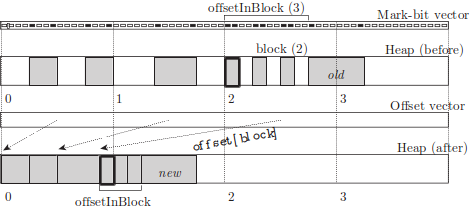
\includegraphics{figures/mrkcmp_2}
  \caption[Ο σωρός (πριν και μετά τη συμπύκνωση) και τα μεταδεδομένα
           που χρησιμοποιεί ο αλγόριθμος Compressor.]
    {Ο σωρός (πριν και μετά τη συμπύκνωση) και τα μεταδεδομένα
     που χρησιμοποιεί ο αλγόριθμος Compressor. Τα bits του διανύσματος
     σήμανσης υποδεικνύουν την αρχή και το τέλος κάθε ζωντανού
     αντικειμένου. Οι λέξεις στο διάνυσμα μετατόπισης αποθηκεύουν
     τη διεύθυνση προς την οποία θα μετακινηθεί το πρώτο ζωντανό
     αντικείμενο του αντίστοιχου μπλοκ. Οι διευθύνσεις προώθησης
     δεν αποθηκεύονται αλλά υπολογίζονται όταν αυτό είναι απαραίτητο
     από τα διανύσματα σήμανσης και μετατόπισης.}
  \label{fig:mrkcmp_2}
\end{figure}

Στην ενότητα
αυτή εξετάζουμε την απλή εκδοχή του αλγορίθμου, όπου και υποθέτουμε πώς
διακόπτεται η εκτέλεση των νημάτων του τροποποιητή κατά την εκτέλεση του
συλλέκτη.

Η λειτουργία του αλγορίθμου στηρίζεται κυρίως στη χρήση βοηθητικών πινάκων ή και
διανυσμάτων. Όπως και πολλοί συλλέκτες, ο αλγόριθμος Compressor χρησιμοποιεί ως
διάνυσμα σήμανσης μια δομή bitmap όπου κάθε bit αντιστοιχεί σε μία λέξη μνήμης. 
Η φάση της σήμανσης θέτει σε λογικό ένα τα bit που αντιστοιχούν στην πρώτη και 
τελευταία λέξη ενός ζωντανού αντικειμένου. Εξετάζοντας τη δομή αυτή, ο συλλέκτης 
είναι σε θέση να προσδιορίσει κατά τη διάρκεια της συμπύκνωσης το μέγεθος ενός 
οιουδήποτε (ζωντανού) αντικειμένου.

Επιπλέον, ο αλγόριθμος χρησιμοποιεί έναν πίνακα όπου αποθηκεύει τις διευθύνσεις
προορισμού των αντικειμένων. Καθώς η αποθήκευση της διεύθυνσης κάθε ενός
αντικειμένου ξεχωριστά θα ήταν απαγορευτική, ο αλγόριθμος διαιρεί το σωρό σε
μικρά, ισομεγέθη μπλοκ με τυπικό μέγεθος 256 ή 512 bytes. Ο πίνακας $offset$
αποθηκεύει τη διεύθυνση προορισμού του πρώτου αντικειμένου για κάθε μπλοκ.
Οι νέες διευθύνσεις των υπολοίπων ζωντανών αντικειμένων μπορούν να υπολογισθούν
με χρήση του πίνακα $offset$ και του διανύσματος σήμανσης. Ομοίως, δοθείσης μιας 
αναφοράς προς ένα αντικείμενο, μπορούμε να υπολογίσουμε το μπλοκ στο οποίο
αντιστοιχεί και επομένως να εξάγουμε τη διεύθυνση προορισμού από την κατάλληλη
καταχώριση στον πίνακα $offset$ και τα bit σήμανσης για αυτό το μπλοκ. Αυτό
επιτρέπει στον αλγόριθμο να αντικαταστήσει τα πολλαπλά περάσματα στο σωρό για
μετακίνηση αντικειμένων και επιδιόρθωση δεικτών με ένα απλό και γρήγορο πέρασμα
του διανύσματος σήμανσης για την κατασκευή του πίνακα $offset$, καθώς και άλλο 
ένα πέρασμα για τη μετακίνηση αντικειμένων και την ενημέρωση των δεικτών 
συμβουλευόμενος τις βοηθητικές αυτές δομές.

\begin{algorithm}[H]
  \caption{Σήμανση-συμπύκνωση: ο αλγόριθμος συμπύκνωσης Compressor}
  \label{alg:mrkcmp3}
  \begin{algorithmic}[1]
    \Procedure{compact}{\null}
      \State \Call{computeLocations}{$HeapStart$, $HeapEnd$, $HeapStart$}
      \State \Call{updateReferencesRelocate}{$HeapStart$, $HeapEnd$}
    \EndProcedure
    \Statex
    \Procedure{computeLocations}{$start$, $end$, $toRegion$}
      \For{$b \gets 0 \; \textbf{to} \; numBits(start, end)-1$}
        \If{$b \bmod BITS\_IN\_BLOCK = 0$}
          \Comment{crossed boundary?}
          \State $offset[block] \gets loc$
          \Comment{first object will be moved to loc}
          \State $block \gets block+1$
        \EndIf
        \If{$bitmap[b] = MARKED$}
          \State $loc \gets loc + BYTES\_PER\_BIT$
          \Comment{advance by size of live objects}
        \EndIf
      \EndFor
    \EndProcedure
    \Statex
    \Procedure{newAddress}{$old$}
      \State $block \gets$ \Call{getBlockNum}{$old$}
      \State \Return{$offset[block]$ $+$ \Call{offsetInBlock}{$old$}}
    \EndProcedure
    \Statex
    \Procedure{updateReferencesRelocate}{$start$, $end$}
      \ForAll{$fld \; \textbf{in} \; Roots$}
        \State $ref \gets *fld$
        \If{$ref \neq \textbf{null}$}
          \State $*fld \gets$ \Call{newAddress}{$ref$}
        \EndIf
      \EndFor
      \State $scan \gets start$
      \While{$scan < end$}
        \State $scan \gets$ \Call{nextMarkedObject}{$scan$}
        \Comment{use the bitmap}  
        \ForAll{$fld \; \textbf{in} \; Pointers(scan)$}
          \Comment{update references}
          \State $ref \gets *fld$
          \If{$ref \neq \textbf{null}$}
            \State $*fld \gets$ \Call{newAddress}{$ref$}
          \EndIf
        \EndFor
        \State $dest \gets$ \Call{newAddress}{$scan$}
        \State \Call{move}{$scan$, $dest$}
      \EndWhile
    \EndProcedure
  \end{algorithmic}
\end{algorithm}

Αφού η ρουτίνα \textproc{computeLocations} υπολογίσει το πίνακα $offset$, η 
ρουτίνα \textproc{updateReferences\-Relocate} ενημερώνει αρχικά τους δείκτες των 
αντικειμένων ριζών. Ο αλγόριθμος Lisp 2 ξεχωρίζει τα περάσματα της μετακίνησης
αντικειμένων και της ενημέρωσης δεικτών, καθώς οι πληροφορίες της μετακίνησης
αποθηκεύονται στο σωρό και χάνονται κατά τη μετακίνηση αντικειμένων. Αντίθετα,
ο αλγόριθμος Compressor μετακινεί τα ζωντανά αντικείμενα και ενημερώνει τους
δείκτες σε ένα μόνο πέρασμα, καθώς οι νέες διευθύνσεις των αντικειμένων
υπολογίζονται εύκολα από τον πίνακα $offset$ και το bitmap σήμανσης και δε
χρειάζεται να αποθηκευθούν στο σωρό. Η ρουτίνα \textproc{newAddress} υπολογίζει
τη νέα διεύθυνση ενός ζωντανού αντικειμένου. Αρχικά υπολογίζει το
μπλοκ στο οποίο ευρίσκεται το αντικείμενο και χρησιμοποιεί την τιμή ως index
στον πίνακα $offset$ ώστε να βρει τη διεύθυνση προορισμού του \textbf{πρώτου}
ενεργού αντικειμένου στο συγκεκριμένο block. Η νέα διεύθυνση του αντικειμένου
προκύπτει προσθέτοντας στην προηγούμενη τιμή το μέγεθος σε λέξεις των ζωντανών
αντικειμένων που προηγούνται του αντικειμένου στο μπλοκ, δεδομένο που υπολογίζει
συμβουλευόμενη το bitmap που αντιστοιχεί στο εν λόγω μπλοκ.


\section{Ανακεφαλαίωση και θέματα προς εξέταση}
\subsection{Είναι απαραίτητη η συμπύκνωση;}
Η συλλογή με σήμανση και εκκαθάριση έχει μικρότερες απαιτήσεις σε μνήμη από ότι 
άλλες τεχνικές όπως η συλλογή με αντιγραφή. Επιπλέον, καθώς δεν μετακινεί 
αντικείμενα, ένας συλλέκτης με σήμανση και εκκαθάριση αρκείται στο να εντοπίσει 
τα προσβάσιμα από τις ρίζες αντικείμενα και να τα σημάνει: δεν τα μεταβάλλει. 
Περιβάλλοντα όπου το σύστημα εκτέλεσης δε μπορεί να παρέχει έγκυρη πληροφορία 
τύπων ώστε να προσδιοριστούν με βεβαιότητα οι μεταβλητές δείκτες δυσχεραίνουν 
τον προσδιορισμό και τη σήμανση αντικειμένων που είναι προσβάσιμα από τις ρίζες 
του τροποποιητή. Παρόλα αυτά, το σημαντικότερο μειονέκτημα ενός συλλέκτη με σήμανση 
και εκκαθάριση είναι η τάση του να κατακερματίζει τη μνήμη. Η χρήση προηγμένων 
τεχνικών για την εκχώρηση μνήμης όπως η χρήση ξεχωριστών συνδεδεμένων λιστών 
ελεύθερων διαφορετικού μεγέθους αντικειμένων (segregated-fits lists) μειώνει την 
πιθανότητα για κατακερματισμό της μνήμης μόνο σε εφαρμογές με μικρές απαιτήσεις σε 
μεγάλα αντικείμενα και με σχετικά μη μεταβλητή αναλογία μεγεθών αντικειμένων. Σε 
μία τυπική εφαρμογή η οποία τρέχει για πολύ χρόνο και στην οποία χρησιμοποιούνται 
αντικείμενα διαφόρων μεγεθών, ο κατακερματισμός που επιφέρει ένας μη-μετακινών 
συλλέκτης αποτελεί πηγή προβλημάτων. Γι αυτόν το λόγο, οι περισσότερες εμπορικές 
υλοποιήσεις της εικονικής μηχανής της γλώσσας Java χρησιμοποιούν μετακινούντες 
συλλέκτες που συμπυκνώνουν το σωρό.

\subsection{Επίδραση στη ρυθμαπόδοση}
Η συλλογή με σήμανση και συμπύκνωση ωστόσο τείνει να είναι πιο αργή από τη 
συλλογή με σήμανση και εκκαθάριση ή τη συλλογή με αντιγραφή. Ο λόγος είναι πώς 
με εξαίρεση με τον αλγόριθμο Compressor, o συλλέκτης πραγματοποιεί πολλαπλά 
περάσματα στο σωρό, με το κάθε πέρασμα να είναι ακριβό. Μια ευρέως χρησιμοποιούμενη
λύση είναι η προσαρμοστική συλλογή σκουπιδιών: ο συλλέκτης εκτελεί τον αλγόριθμο
με σήμανση και εκκαθάριση και προσφεύγει στον αλγόριθμο με σήμανση και συμπύκνωση
όταν οι μετρικές κατακερματισμού υποδεικνύουν πώς η αλλαγή θα είναι επικερδής.
\cite{DBLP:conf/jvm/Printezis01, DBLP:conf/iwmm/SomanKB04}.   

\subsection{Μακρόβια αντικείμενα}
Δεν είναι ασυνήθιστο για αντικείμενα που ζουν πολύ ή είναι αθάνατα (δηλαδή ζουν
καθόλη τη διάρκεια εκτέλεσης του τροποποιητή) να συσσωρεύονται στην αρχή του
σωρού από μετακινούντες συλλέκτες. Οι συλλέκτες με αντιγραφή διαχειρίζονται μη
αποδοτικά τα αντικείμενα αυτά, αντιγράφοντάς τα συνέχεια από τον ένα ημιχώρο
στον άλλον. Από την άλλη πλευρά, οι γενεαλογικοί συλλέκτες (τους οποίους
εξετάζουμε στο κεφάλαιο 6), τα προωθούν σε διαφορετικό τμήμα του σωρού, το
οποίο και συλλέγεται σπανίως. Η γενεαλογική συλλογή σκουπιδιών ωστόσο δεν
ενδείκνυται πάντα και ιδιαίτερα όταν ο σωρός είναι σχεδόν γεμάτος. Επίσης δε
λύνει το πρόβλημα αν τα αντικείμενα βρίσκονται ήδη αποθηκευμένα στην παλαιότερη
γενεά. Η συλλογή με σήμανση και συμπύκνωση μπορεί να επιλέξει τη μη συμπύκνωση
αυτού του ``ιζήματος''. O Hanson \cite{DBLP:journals/spe/Hanson77} πρώτος
παρατήρησε την εμφάνιση του προβλήματος στο σύστημα SITBOL, το οποίο αποτελούσε
μία υλοποίηση της γλώσσας SNOBOL4 για αρχιτεκτονική DEC-10. O Hanson πρότεινε
τη δυναμική μέτρηση του μεγέθους του 'ιζήματος' και τη μη συλλογή αυτού εκτός
και αν είναι τελείως απαραίτητη, με τίμημα ένα μικρό ποσοστό κατακερματισμού.

\subsection{Τοπικότητα}
Όπως είδαμε, οι συλλέκτες με σήμανση και συμπύκνωση μπορεί να διατηρούν τη
διάταξη των αντικειμένων στο σωρό είτε να τα αναδιατάσσουν τυχαία. Παρότι
οι δεύτεροι είναι ταχύτεροι και χωρίς κόστος σε χώρο, η τοπικότητα του
τροποποιητή ενδέχεται να καταστραφεί τελείως από την τυχαία διάταξη των
αντικειμένων. Η ολισθαίνουσα συμπύκνωση έχει τέλος ένα ακόμη πλεονέκτημα:
η ανάκτηση της συνολικής μνήμης που καταλαμβάνεται από αντικείμενα μετά
από ένα συγκεκριμένο όριο στο σωρό δύναται να ανακτηθεί αμέσως με μία απλή
μείωση του δείκτη $free$.

\subsection{Περιορισμοί}
Στη βιβλιογραφία έχει προταθεί μια πληθώρα αλγορίθμων συλλογής
με σήμανση και συμπύκνωση. Πολλοί από αυτούς ωστόσο έχουν
ιδιότητες μη επιθυμητές και σε αρκετές περιπτώσεις απαράδεκτες.
Ένα από τα ζητήματα αφορά το κόστος σε χώρο που επιβάλλει
η ανάγκη αποθήκευσης των διευθύνσεων προώθησης (παρότι αυτό
είναι μικρότερο από το αντίστοιχο κόστος της συλλογής με
αντιγραφή). Μερικοί αλγόριθμοι συμπύκνωσης επιβάλλουν περιορισμούς
στον τροποποιητή. Απλοί αλγόριθμοι όπως ο Two-Finger μπορούν
να διαχειριστούν μόνο αντικείμενα του ίδιου μεγέθους. Εφόσον
λοιπόν είναι δυνατός ο διαχωρισμός των αντικειμένων με βάση
το μέγεθός τους, σε ποιο βαθμό είναι απαραίτητη η συμπύκνωση;
Τέλος, οι περισσότεροι αλγόριθμοι συμπύκνωσης αποκλείουν τη
χρήση εσωτερικών δεικτών: ο αλγόριθμος Two-Finger αποτελεί
εξαίρεση.
\end{greek}
